\documentclass[tikz, border=0 3pt 0 3pt]{standalone}

\begin{document}
   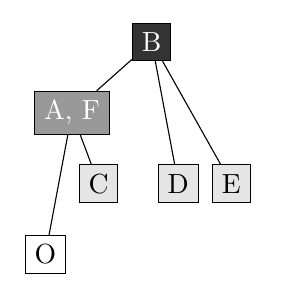
\begin{tikzpicture}[scale=0.9]
      \tikzset{every node/.style={draw=black, rectangle}}
      \path[use as bounding box] (-1.75,0.2) rectangle (1.75,-3.2);
      % \foreach \x in {0,1,...,3} {
      %   \draw[gray, dashed] (-1.75,-\x) -- (1.75,-\x);
      % }

      \node[white, draw=black, fill=black!80] {B}
      [level distance=1cm, sibling distance=.75cm]
      child { node[white, draw=black, fill=black!40] {A, F} [sibling distance=.75cm]
        child[level distance=2cm] { node[fill=white] {O} }
        child { node[fill=black!10] {C} }
      }
      child[missing]
      child[level distance=2cm] { node[fill=black!10] {D} }
      child[level distance=2cm] { node[fill=black!10] {E} }
      ;
    \end{tikzpicture}
\end{document}